% Пример заготовки для презентации с использованием класса Beamer LaTeX.
% Версия от 09 ноября 2018 года.
\documentclass[12pt,a4paper,mathserif]{beamer}
\usepackage[utf8x]{inputenc}
\usepackage{ucs}
\usepackage[T2A]{fontenc}
\usepackage[english,russian]{babel}
\usepackage{amsmath}
\usepackage{amsfonts}
\usepackage{amssymb}
\usepackage{mathtext}
\usepackage{graphicx}
\usepackage{enumerate}
\usepackage{multirow}
\usepackage{ragged2e}
% Пакет для оформления исходного кода
\usepackage{minted}
\usepackage{adjustbox}
\justifying
\renewcommand{\raggedright}{\leftskip=0pt \rightskip=0pt plus 0cm}
\setbeamertemplate{caption}[numbered]

\usetheme {Madrid}
\usecolortheme [RGB={85, 107, 47}]{structure} %Dark Olive Green

\author[Лаптев А.В.]{{Cтудент 5.306М группы: Лаптев А.~В.}\\
{Научный руководитель: Калачев А.~В.}}
\title[Барнаул 2025]{Автоматизация решения CAPTCHA в текстовом формате}
% \subtitle{Отчет по научно-исследовательской работе}

\begin{document}
\begin{frame}
\maketitle
\end{frame}

\begin{frame}{Цель и задачи работы}
    \setlength{\parindent}{0.5cm}
    Целью работы является: разработать, реализовать и протестировать программу для автоматизированного распознавания текстовых CAPTCHA.

    Задачи, которые необходимо решить для достижения цели:

    \begin{enumerate}
        \item изучить принципы реализации текстовых CAPTCHA на основе открытых источников (допустимые символы, применяемые искажения);
        \item выбрать архитектуру нейронной сети, наиболее подходящую для распознавания CAPTCHA;
        \item подготовить датасет изображений CAPTCHA с учётом возможных искажений;
        \item обучить нейронную сеть с достаточной точностью;
        \item протестировать модель на тестовом наборе данных и оценить её эффективность.
    \end{enumerate}
\end{frame}

\begin{frame}{Современная реализация текстовых CAPTCHA}
    \setlength{\parindent}{0.5cm}
    Текстовые CAPTCHA обычно состоят из букв и цифр. Зачастую используются символы латинского алфавита (как прописные, так и строчные) и цифры от 0 до 9. Рекомендуемый набор символов в генераторах на некоторых CRM платформах выглядит следующим образом: ABCDEFGHJKLMNPQRSTWXYZ23456789. Длина последовательности символов обычно составляет от 4 до 8 символов.

    Для усложнения автоматического распознавания текстовые \\CAPTCHA подвергаются различным искажениям:
    \begin{enumerate}
        \item геометрические искажения;
        \item перекрытие символов;
        \item добавление шума;
        \item сложные фоны;
        \item нелинейные искажения.
    \end{enumerate}
\end{frame}

\begin{frame}{Подготовка датасета с изображениями}
    \setlength{\parindent}{0.5cm}
    Для эффективного обучения необходимо, чтобы набор данных соответствовал следующим требованиям:

    \begin{enumerate}
        \item достаточное количество изображений для каждого символа;
        \item разнообразие данных, включающее:
        \begin{enumerate}
            \item различные углы наклона символов;
            \item вариативность написания символов и их искажения;
            \item наличие побочных визуальных элементов;
            \item использование различных шрифтов.
        \end{enumerate}
        \item переменная длина последовательностей символов.
    \end{enumerate}

    Для генерации синтетических CAPTCHA использовалась библиотека captcha на языке python. Данная библиотека поддерживает генерацию изображений с пользовательскими шрифтами и различными эффектами искажений, что исключает необходимость привлечения дополнительных инструментов.
\end{frame}

\newlength\someheight
\setlength\someheight{3,5cm}

\begin{frame}[fragile]{{Блок кода для генерации CAPTCHA}}
    \begin{adjustbox}{width=\textwidth,height=\someheight,keepaspectratio}
    \begin{minipage}{1.1\linewidth}
    \begin{minted}{Python}
        from captcha.image import ImageCaptcha
        from random import randint, shuffle
        import numpy as np
        import os
        from textcaptcha.preprocessing_image import preprocessing_image
        
        def generate_image(path_to_file: str, alphabet: list,
            number_of_start:int, number_of_captcha: int,
            size_of_image: tuple) -> list:
            # Генерация текстовых captcha
            text = ImageCaptcha(size_of_image[0], size_of_image[1],
            ['./fonts/arial.ttf', './fonts/comic.ttf', './fonts/cour.ttf',
            './fonts/georgia.ttf'])
            # Структура возвращаемого списка:
            # [filename, label, (width, height)]
            filenames = []
            for _ in range(number_of_start, number_of_captcha):
                captcha_text = [alphabet[randint(0, len(alphabet) - 1)]
                for _ in range(randint(4, 7))]
                shuffle(captcha_text)
                text.write(''.join(captcha_text),
                f'{path_to_file}/{"".join(captcha_text)}.png')
                filenames.append(
                    [f'{path_to_file}/{"".join(captcha_text)}.png',
                    ''.join(captcha_text)]
                )
            return filenames
    \end{minted}
    \end{minipage}
    \hfill
    \begin{minipage}{1.1\linewidth}
    \begin{minted}{Python}
            if __name__ == '__main__':
                # Алфавит допустимых символов
                alphabet = 'ABCDEFGHJKLMNPQRSTWXYZ023456789'
                # Создание директории для хранения полноценных
                # синтетических текстовых captcha
                path_to_dataset = '../datasets/captcha'
                if not os.path.isdir(path_to_dataset):
                    os.mkdir(path_to_dataset)
                # Создаем датасет из нужного полноценных
                # синтетических captcha длиной от 4 до 7
                # символов размером 250х60
                filenames = generate_image(path_to_dataset,
                list(alphabet), 0, 100000, (250, 60))
            
                # Предобработка изображений
                preprocessing_image(filenames)
            
                # Для отладки без создания датасета с нуля
                numpy_data = np.array(filenames, dtype=object)
                np.save('data.npy', numpy_data)
    \end{minted}
    \end{minipage}
    \end{adjustbox}
\end{frame}

\begin{frame}{Предобработка датасета с изображениями}
    \setlength{\parindent}{0.5cm}
    После создания изображений все они прошли этапы предобработки, направленные на улучшение качества данных и повышение эффективности обучения модели.

    Примеры сгенерированных и предобработанных CAPTCHA приведены на рисунке ниже:

    \begin{figure}[H]
        \centering
        \begin{minipage}[h]{0.45\linewidth}
            \center{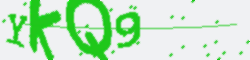
\includegraphics[width=1\linewidth]{imgs/YKQ9.png}} \\
        \end{minipage}
        \begin{minipage}[h]{0.45\linewidth}
            \center{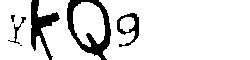
\includegraphics[width=1\linewidth]{imgs/out.png}} \\
        \end{minipage}
        \caption{Изображение CAPTCHA и результат обработки.}
        \label{fig:example-captcha}
    \end{figure}
\end{frame}

\begin{frame}{Выбор эффективной модели}
    \setlength{\parindent}{0.5cm}
    Для распознавания текста с переменной длиной последовательности в задачах CAPTCHA наиболее часто применяются следующие архитектуры нейронных сетей:

    \begin{enumerate}
        \item оптическое распознавание символов (OCR);
        \item рекуррентные сверточные нейронные сети (CRNN);
        \item архитектуры последовательного обучения (Seq-to-Seq).
    \end{enumerate}
    
    На начальных этапах экспериментов Seq-to-Seq-модель показала наилучшие результаты среди рассмотренных вариантов. В отличие от OCR- и CRNN-моделей, данная архитектура смогла достичь более высокой точности распознавания последовательностей символов, что обусловлено применением механизма внимания. Дальнейшая работа с моделью была сосредоточена на её оптимизации и улучшении параметров обучения.
\end{frame}

\begin{frame}{Seq-to-Seq модель. Функция потерь}
    \begin{figure}[H]
        \centering
        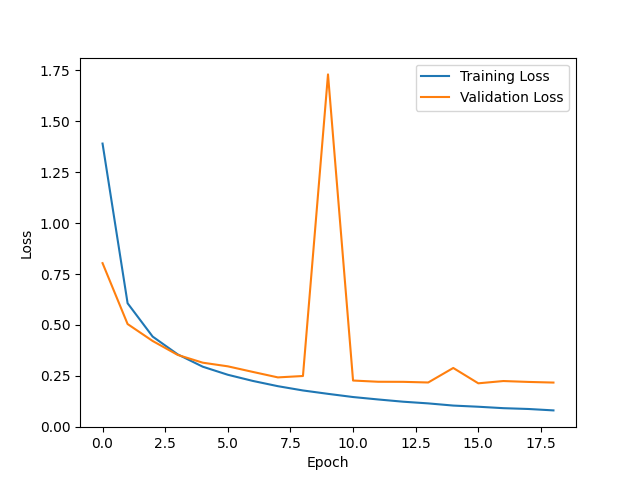
\includegraphics[width=0.7\linewidth]{imgs/Model_loss.png}
        \caption{График изменения значений функции потерь.}
        \label{fig:loss}
    \end{figure}
\end{frame}

\begin{frame}{Seq-to-Seq модель. Точность предсказаний}
    \begin{table}[H]
    \centering
    \caption{Точность предсказаний для последовательностей от 4 до 7 символов.}
    \begin{tabular}{|l|l|}
        \hline
        Длина последовательности & Точность распознавания \\
        \hline
        4 символа & 0.9305 \\
        \hline
        5 символов & 0.7450 \\
        \hline
        6 символов & 0.4575 \\
        \hline
        7 символов & 0.1915 \\
        \hline
    \end{tabular}
    \label{tab:probability}
\end{table}
\end{frame}

\begin{frame}{Seq-to-Seq модель. Матрица ошибок}
    \begin{figure}[H]
        \centering
        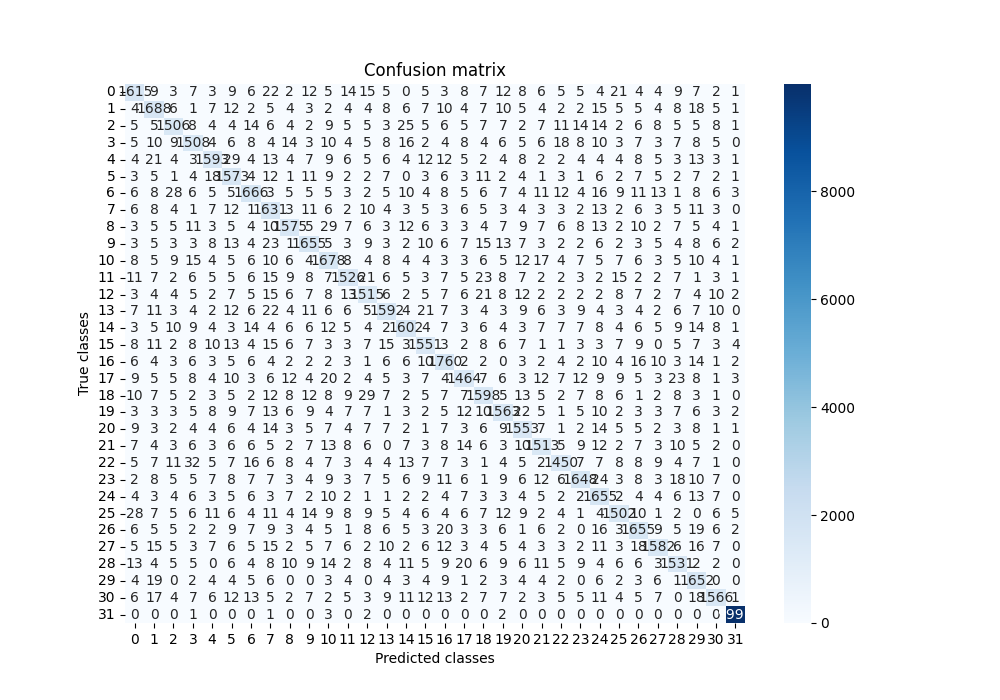
\includegraphics[width=0.85\linewidth]{imgs/Confusion_matrix.png}
        \caption{Матрица ошибок для обученной модели.}
        \label{fig:cm}
    \end{figure}
\end{frame}

\begin{frame}{Заключение}
    \setlength{\parindent}{0.5cm}
    В ходе выполнения работы были решены задачи:
    \begin{enumerate}
        \item определен набор допустимых символов и искажений для создания датасета с текстовыми CAPTCHA;
        \item выбрана модель нейронной сети Seq-to-Seq для распознавания текста с CAPTCHA;
        \item подготовлен датасет из 100 000 изображений для обучения и тестирования модели нейронной сети;
        \item обучена модель на изображениях с различной длиной последовательностей символов;
        \item протестирована работа модели на тестовых изображениях.
    \end{enumerate}
    
    В результате выполнения работы была создана модель, для распознавания текстовых CAPTCHA различной длины последовательности символов.
\end{frame}

\end{document}
